\documentclass{beamer}
\usetheme{CambridgeUS}
\usefonttheme{structurebold}
\usefonttheme{serif}
\usefonttheme{professionalfonts}
\usefonttheme{structureitalicserif}


\usepackage{graphicx}
\usepackage{tikz}
\usepackage{xcolor}
\usepackage{booktabs}
\usepackage{caption}
\usepackage{subcaption}
\usepackage{tikz}
\usetikzlibrary{positioning}
\usetikzlibrary{arrows.meta}        % <-- added: arrow tips for the flow diagram
\usepackage{array}   
\usepackage[table]{xcolor} 
\usepackage{booktabs}
\usepackage{float} 
\usepackage{colortbl}   
\usepackage{tcolorbox}
\usepackage[utf8]{inputenc}
\usepackage[T1]{fontenc}
\usepackage{enumitem}
\usepackage{amssymb}
\usepackage{textcomp}
\usepackage{helvet}
\renewcommand{\familydefault}{\sfdefault}


% ---- palette -----------------------------------------------
\definecolor{kgreen}{RGB}{20,94,66}      % deep green (titles, accents)
\definecolor{kgreenlt}{RGB}{233,243,238}  % pale green (message strip)
\definecolor{ktext}{RGB}{38,44,41}



\definecolor{darkgreen}{RGB}{0, 100, 70}
\definecolor{softgreen}{RGB}{210, 235, 220}
\definecolor{ashgray}{RGB}{242, 242, 242}
\definecolor{softgray}{RGB}{125, 145, 135}

\definecolor{emerald}{RGB}{0, 140, 90}
\definecolor{lightemerald}{RGB}{225, 245, 235}

\definecolor{emerald1}{RGB}{0, 85, 55}
\definecolor{lightemerald1}{RGB}{215, 240, 225}




% General colors
\setbeamercolor{palette primary}{fg=black, bg=softgray}
\setbeamercolor{palette secondary}{fg=darkgreen}
\setbeamercolor{palette tertiary}{bg=darkgreen, fg=white}
\setbeamercolor{title}{fg=white,bg=darkgreen}
\setbeamercolor{normal text}{bg=, fg=black}
\setbeamercolor{structure}{fg=darkgreen}

% Frame title
\setbeamercolor{frametitle}{bg=softgreen, fg=darkgreen}

% Blocks
\setbeamercolor{block title}{bg=darkgreen!25, fg=black}
\setbeamercolor{block body}{bg=white, fg=black}

% Itemize bullets
\setbeamerfont{enumerate item}{series=\bfseries} % bold numbers
\setbeamercolor{enumerate item}{fg=darkgreen}   % change number color

\setbeamerfont{itemize item}{series=\bfseries} % bold bullet
\setbeamercolor{itemize item}{fg=darkgreen}   % bullet color


% Section in TOC
\setbeamercolor{section in toc}{fg=darkgreen}

% Footer (optional)
\setbeamercolor{author in head/foot}{bg=darkgreen, fg=white}

% Frame title: bold & upright
\setbeamerfont{frametitle}{series=\bfseries, shape=\upshape}

\setbeamertemplate{caption}[numbered]
\setbeamerfont{caption name}{size=\tiny}
\setbeamerfont{caption}{size=\tiny}




\definecolor{hicolor}{HTML}{C0392B}
\newcommand{\hi}[1]{\textbf{\textcolor{hicolor}{#1}}}

% ---- emphasis + key message --------------------------------
\newcommand{\key}[1]{\textcolor{kgreen}{\bfseries #1}}
\newcommand{\keymsg}[1]{%
	\vskip0.4em
	\begin{beamercolorbox}[wd=\textwidth,sep=0.7em,rounded=false]{}%
		\colorbox{kgreenlt}{\parbox{\dimexpr\textwidth-1.4em\relax}{%
				{\bfseries\color{kgreen}Key Message.\ }#1}}%
\end{beamercolorbox}}


\setlist[itemize]{label=\textbullet}
\setlist[enumerate]{label=\arabic*., leftmargin=*}


% ---- helpers added for these slides ------------------------
\newcommand{\dropcol}{hicolor}      % red   -> excluded / removed
\newcommand{\keepcol}{emerald1}     % green -> retained / used


\title[Elephant Movement in Kaudulla]{\centering \LARGE Elephant Movement in Kaudulla: What the Data Tells Us}


\institute[SCS-USJ]{
	{Statistical Consulting Service \par}
	{Department of Statistics \par}
	{Faculty of Applied Sciences \par}
	{University of Sri Jayewardenepura \par}
	{Nugegoda \par}
	{Sri Lanka}
}
\date[\today]{\today}




\begin{document}
	
	
	
	
	\begin{frame}
		\titlepage
	\end{frame}
	
	
	\begin{frame}{What This Project Is}
		\vspace{0.3em}
		
		\begin{block}{}
			The Department already collars and tracks elephants in Kaudulla.
			\key{This project turns that existing GPS data into patterns the raw records do not show.}
		\end{block}
		
		\vspace{0.6em}
		\textbf{What we did with the data}
		\vspace{0.3em}
		
		\begin{enumerate}
			\setlength{\itemsep}{0.45em}
			\item Monitoring missing data
			\item Analysis of elephants' movements
			\item Climate and vegetation data analysis
			\item Checking elephant movement anomalies
		\end{enumerate}
		
	\end{frame}
	
	% ============================================================
	\begin{frame}{The Data We Worked With}
		\vspace{0.4em}
		\centering
		\resizebox{\textwidth}{!}{%
			\begin{tabular}{@{}c>{\raggedright\arraybackslash}p{3.3cm}>{\raggedright\arraybackslash}p{2.5cm}>{\raggedright\arraybackslash}p{2.3cm}>{\raggedright\arraybackslash}p{3.1cm}@{}}
				\toprule
				\rowcolor{lightemerald}
				\textbf{\#} & \textbf{Dataset} & \textbf{Time resolution} & \textbf{Period} & \textbf{Size} \\
				\midrule
				1 & Elephant GPS tracking & \key{Hourly} & Jul 2024 -- Jun 2026 & 16,747 records, 15 elephants \\
				2 & Climate & \key{Monthly} & 2017 -- 2025 & 9 variables $\times$ 9 years \\
				3 & NDVI vegetation classification & \key{Annually} & 2018 -- 2026 & 5 density classes \\
				\bottomrule
		\end{tabular}}
		
		
	\end{frame}
	
	% ============================================================
	\begin{frame}{Variables Used from Each Dataset}
		\vspace{0.4em}
		
		\begin{columns}[T]
			
			% ---------- tracking ----------
			\begin{column}{0.32\textwidth}
				\begin{tcolorbox}[colback=lightemerald, colframe=darkgreen, boxrule=0.9pt,
					arc=2pt, left=3pt, right=3pt, top=3pt, bottom=3pt]
					{\scriptsize\textbf{\color{darkgreen}1. GPS Tracking}}\\[1pt]
					{\tiny\textit{Hourly}}\\[4pt]
					{\tiny
						\begin{tabular}{@{}ll@{}}
							\texttt{collar\_id} & Collar number \\[1.5pt]
							\texttt{name}       & Elephant name \\[1.5pt]
							\texttt{sex}        & Male / Female \\[1.5pt]
							\texttt{date}       & Date of fix \\[1.5pt]
							\texttt{time}       & Time of fix \\[1.5pt]
							\texttt{lat}        & Latitude \\[1.5pt]
							\texttt{lon}        & Longitude \\
					\end{tabular}}
				\end{tcolorbox}
			\end{column}
			
			% ---------- climate ----------
			\begin{column}{0.30\textwidth}
				\begin{tcolorbox}[colback=ashgray, colframe=softgray, boxrule=0.9pt,
					arc=2pt, left=3pt, right=3pt, top=3pt, bottom=3pt]
					{\scriptsize\textbf{\color{darkgreen}2. Climate}}\\[1pt]
					{\tiny\textit{Monthly}}\\[4pt]
					{\tiny
						\textbf{Rainfall}\\[1pt]
						\texttt{PRECTOTCORR}\\[1pt]
						Precipitation Corrected (mm)\\[6pt]
						\textbf{Temperature}\\[1pt]
						\texttt{T2M}\\[1pt]
						Temperature at 2 Meters ($^\circ$C)}
				\end{tcolorbox}
			\end{column}
			
			% ---------- vegetation ----------
			\begin{column}{0.34\textwidth}
				\begin{tcolorbox}[colback=lightemerald1, colframe=emerald1, boxrule=0.9pt,
					arc=2pt, left=3pt, right=3pt, top=3pt, bottom=3pt]
					{\scriptsize\textbf{\color{emerald1}3. NDVI Vegetation}}\\[1pt]
					{\tiny\textit{Annually}}\\[4pt]
					{\tiny
						\textbf{\% cover by density class}\\[2pt]
						$\bullet$~Non-vegetation\\[1pt]
						$\bullet$~Shrubs \& degraded grasslands\\[1pt]
						$\bullet$~Sparse or stressed vegetation\\[1pt]
						$\bullet$~Moderate canopy coverage\\[1pt]
						$\bullet$~High density forest\\[5pt]
						\textbf{\% cover by plant health}\\[2pt]
						$\bullet$~Very healthy plant\\[1pt]
						$\bullet$~Moderate healthy plant\\[1pt]
						$\bullet$~Unhealthy plant}
				\end{tcolorbox}
			\end{column}
			
		\end{columns}
	\end{frame}
	
	% ============================================================
	\begin{frame}{Dataset 1: GPS Tracking Data}
		\vspace{0.2em}
		
		\begin{center}
			\resizebox{\textwidth}{!}{%
				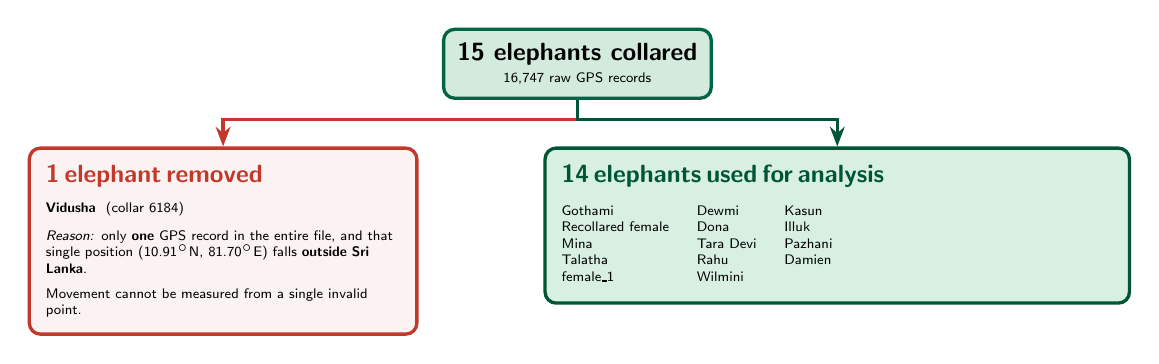
\begin{tikzpicture}[font=\tiny]
					
					% ---- top: total ----
					\node[draw=darkgreen, very thick, rounded corners, fill=softgreen,
					inner sep=5pt, align=center] (T) at (0,3.1)
					{\textbf{\small 15 elephants collared}\\[2pt] 16,747 raw GPS records};
					
					% ---- left: removed ----
					\node[draw=hicolor, very thick, rounded corners, fill=hicolor!6,
					text width=4.5cm, align=left, inner sep=6pt, anchor=north] (L) at (-4.5,2.05)
					{\textbf{\color{hicolor}\small 1 elephant removed}\\[5pt]
						\textbf{Vidusha} \ (collar 6184)\\[4pt]
						\textit{Reason:} only \textbf{one} GPS record in the
						entire file, and that single position
						(10.91$^\circ$N, 81.70$^\circ$E) falls
						\textbf{outside Sri Lanka}.\\[3pt]
						Movement cannot be measured from a
						single invalid point.};
					
					% ---- right: retained ----
					\node[draw=emerald1, very thick, rounded corners, fill=lightemerald1,
					text width=7.0cm, align=left, inner sep=6pt, anchor=north] (R) at (3.3,2.05)
					{\textbf{\color{emerald1}\small 14 elephants used for analysis}\\[5pt]
						\begin{tabular}{@{}l@{\hspace{10pt}}l@{\hspace{10pt}}l@{}}
							Gothami   & Dewmi     & Kasun   \\
							Recollared female & Dona & Illuk \\
							Mina      & Tara Devi & Pazhani \\
							Talatha   & Rahu      & Damien  \\
							female\_1 & Wilmini   &         \\
					\end{tabular}};
					
					\draw[-{Stealth[length=2.5mm]}, hicolor, very thick]  (T.south) -- ++(0,-0.25) -| (L.north);
					\draw[-{Stealth[length=2.5mm]}, emerald1, very thick] (T.south) -- ++(0,-0.25) -| (R.north);
					
			\end{tikzpicture}}
		\end{center}
		
		\vspace{0.4em}
		\begin{center}
			{\footnotesize After cleaning: \key{16,735 valid GPS records} across \key{14 elephants}.}
		\end{center}
		
	\end{frame}
	
	% ============================================================
	\begin{frame}{Cleaning Criteria Applied to the Tracking Data}
		\vspace{0.2em}
		\centering
		\tiny
		\begin{tabular}{@{}c>{\raggedright\arraybackslash}p{2.3cm}>{\raggedright\arraybackslash}p{3.2cm}>{\raggedright\arraybackslash}p{3.0cm}c@{}}
			\toprule
			\rowcolor{lightemerald}
			\textbf{\#} & \textbf{Criterion} & \textbf{Rule applied} & \textbf{Why} & \textbf{Removed} \\
			\midrule
			1 & Name correction & Collar 6165 ``\ldots'' renamed \texttt{female\_1} & The unnamed animal needed a stable label & --- \\
			2 & Valid timestamp & Date and time must be readable & A corrupt time cannot be placed on the timeline & 0 \\
			3 & Coordinates present & Latitude and longitude not blank & No position means no movement & 0 \\
			4 & Inside Sri Lanka & Lat 5.9--9.9, Lon 79.5--81.9 & Impossible positions from poor satellite geometry & \hi{4} \\
			5 & GPS accuracy & HDOP $\leq$ 10 & High HDOP means an error of hundreds of metres & \hi{8} \\
			\bottomrule
		\end{tabular}
		
		\vspace{0.8em}
		\raggedright
		{\scriptsize
			$\bullet$~\key{Total removed: 12 records out of 16,747} $=$ \key{0.07\%}\\[3pt]
			$\bullet$~\key{No interpolation applied.} Missing hours were left blank, not filled
			with estimated positions.}
		
	\end{frame}
	
	% ============================================================
	\begin{frame}{Data Availability by Elephant}
		\vspace{0.3em}
		\centering
		\resizebox{\textwidth}{!}{%
			\begin{tabular}{@{}llccrrrrr@{}}
				\toprule
				\rowcolor{lightemerald}
				\textbf{Collar} & \textbf{Name} & \textbf{Sex} & \textbf{Start} & \textbf{End} & \textbf{Days} & \textbf{Fixes} & \textbf{Expected} & \textbf{\% avail.} \\
				\midrule
				6119 & Pazhani & F & 2025-09-07 & 2025-09-09 & 2.0 & 50 & 50 & 100.0 \\
				6182 & Damien & M & 2025-09-08 & 2025-09-09 & 0.6 & 15 & 15 & 100.0 \\
				6156 & Wilmini & F & 2024-10-16 & 2024-10-22 & 6.5 & 131 & 157 & 83.4 \\
				6123 & Rahu & M & 2025-10-20 & 2025-11-13 & 24.0 & 357 & 577 & 61.9 \\
				6155 & Gothami & F & 2024-08-23 & 2025-11-11 & 444.9 & 5,373 & 10,678 & 50.3 \\
				6129 & Kasun & M & 2025-07-13 & 2025-07-30 & 18.0 & 193 & 432 & 44.7 \\
				6121 & Recollared female & F & 2024-08-25 & 2026-06-17 & 660.9 & 5,127 & 15,862 & 32.3 \\
				6165 & female\_1 & F & 2024-08-23 & 2025-07-23 & 334.0 & 2,354 & 8,018 & 29.4 \\
				6144 & Illuk & M & 2025-06-22 & 2025-07-20 & 27.9 & 87 & 671 & 13.0 \\
				6139 & Mina & F & 2024-07-14 & 2025-10-27 & 470.0 & 1,045 & 11,280 & 9.3 \\
				6114 & Talatha & F & 2024-07-18 & 2025-10-27 & 466.2 & 853 & 11,191 & 7.6 \\
				6131 & Dona & F & 2024-09-09 & 2025-08-06 & 331.0 & 464 & 7,946 & 5.8 \\
				6154 & Dewmi & F & 2024-11-09 & 2025-11-28 & 384.0 & 451 & 9,216 & 4.9 \\
				6179 & Tara Devi & F & 2024-07-22 & 2025-10-09 & 443.9 & 235 & 10,654 & \hi{2.2} \\
				\bottomrule
		\end{tabular}}
		
		\vspace{0.5em}
		
	\end{frame}
	
	
	\begin{frame}{Landscape-Level Movement}
		
		\Large
		
		All tracked elephants use a common landscape centered around the \textbf{Kaudulla Reservoir}, with many also moving towards the \textbf{Ralapanawa Nature Reserve}.
		
	\end{frame}
	
	\begin{frame}{Movement Pattern Observation}
		
		\Large
		
		\begin{itemize}
			\item An interesting observation is that \textbf{Gothami} and \textbf{female\_1} show very similar movement patterns during September, October, and November 2024.
			
			\vspace{0.5cm}
			
			\item \textbf{Dona} mainly stayed in the northern part of the park, while \textbf{Recollared\_Female} showed a unique pattern with frequent visits to both the railway track area and the upper region.
			
		\end{itemize}
	\end{frame}
		
		
	\begin{frame}{Home Range \& Movements}
		\begin{itemize}
			\item Kasun and Rahu demonstrated the widest directional movement, whereas Damian and Iluk followed more focused movement routes, indicating individual differences in space use.
			
			\vspace{0.5cm}
			
			\item Female elephants displayed balanced movement in nearly all directions, suggesting widespread use of available habitat with only minor variation in directional frequency.
			
			\vspace{0.5cm}
			
			\item The per-elephant summary table provides an overall comparison of tracking duration, movement, home range size, GPS data availability, and movement speed for each elephant, allowing individual movement behavior and space-use patterns to be compared across the study population.
			
			
	\end{itemize}	
	\end{frame}
		
		
		\begin{frame}{Climate-Driven Spatial Patterns of the Re-collared Female}
			\begin{itemize}
				\item Her movement pattern indicates that she tends to stay farther from the reservoir during periods of lower daytime and nighttime temperatures.
				
				\vspace{0.5cm}
				
				\item Her locations in December 2024 and December 2025 were geographically very similar, with both occurring away from the reservoir. These observations were recorded under the same rainfall category, indicating consistency in habitat use under similar rainfall conditions in same period of year.
			\end{itemize}
		\end{frame}
		
		\begin{frame}{Comparison of Daytime and Nighttime Locations}
			\Large
			\begin{itemize}
				\item Day and night GPS points overlap considerably, indicating stable
				home ranges rather than different day/night territories.
				
				\vspace{0.5cm}
				
				\item Although elephants appear to use areas slightly further into the reservoir during the daytime than at night.
			\end{itemize}
			
		\end{frame}
			
			
			\begin{frame}{Comparison of Hot and Cool Season Locations}
			\footnotesize
			\begin{itemize}
				\item During the hot season, elephants appeared to move further into the reservoir.
				\item Some elephants, such as Gothami and Dewmi, occupied more northerly areas during the cool season, indicating that their locations were relatively more southerly during the hot season.
				\item The Recollared Female had the most balanced hot–cool dataset (67\%, 33\%) among the well-tracked elephants. She showed a distinct seasonal pattern in 2024 and 2025, with her cool-season locations shifting away from the reservoir towards the Trincomalee railway line. However, this pattern was not evident in 2026.
				\item During the hot season of both 2025 and 2026, Recollared female's GPS locations appeared to be more frequently concentrated near a paddy field.
				\item \textbf{Caution:} Since the dataset was imbalanced across seasons, with most elephants tracked only during either the hot or the cool season, seasonal comparisons are limited. Although a few individuals appear to shift their locations between hot and cool periods, the evidence is insufficient to draw strong conclusions about seasonal movement.
				
			\end{itemize}
		\end{frame}
		
		\begin{frame}{Comparison of Heavy and Low Rainfall Locations}
			\begin{itemize}
				\item Most elephants occupied similar areas during both heavy and low rainfall periods.
				
				\vspace{0.5cm}
				
				\item Gothami showed a slight northward shift under low rainfall conditions compared with heavy rainfall periods.
				
				\vspace{0.5cm}
				
				\item Some individuals were only tracked in one rainfall condition, so
				comparisons were limited.
			\end{itemize}
			\vspace{6pt}
			
		\end{frame}
		
		
		% ============================================================
		
		
		\begin{frame}{Vegetation Dynamics and Elephant Movement Patterns}
			\begin{itemize}
				\item Vegetation changed slightly across the three years.
				
				\vspace{0.5cm}
				
				\item 2026 had the highest canopy cover, but also the highest proportion of
				non-vegetated land. This is the key vegetation signal that connects
				to elephant behavior, but 2026 data is only available for recollared
				female.
				
				\vspace{0.5cm}
				
				\item Across 2024 and 2025, most elephants exhibited stable home ranges. However, the Recollared Female showed a noticeable shift away from the reservoir area in 2026 compared with 2024 and 2025.
				
			\end{itemize}
		\end{frame}
		
		
		
		
		
		\begin{frame}{Monthly Home Range variation}
			\begin{itemize}
				\item The Recollared Female had the most complete monthly data and showed the widest monthly home range (4.27 km) in April 2025, at the beginning of the hot season. 
				
				\vspace{0.5cm}
				
				\item For the remaining elephants, monthly data were concentrated mainly between June and December. Within this period, several elephants exhibited larger home ranges around October–November.
			\end{itemize}
		
	\end{frame}
	
	
	
	
\end{document}